\documentclass[UTF8,12pt]{ctexart}
\usepackage[a4paper,margin=24mm]{geometry}
\usepackage{amsmath,amssymb,bm,graphicx,adjustbox}
\newcommand{\fitmath}[1]{\begin{adjustbox}{max width=\linewidth}$\displaystyle #1$\end{adjustbox}}
\setlength{\parindent}{0pt}
\setlength{\parskip}{.7em}
\sloppy
\allowdisplaybreaks
\begin{document}
\section*{1993 年考研数学三 · 参考答案}
\subsection*{1993 年真题参考答案（试卷 IV）}

\subsection*{一、填空题}

（1）\(\displaystyle \dfrac{\displaystyle 6}{\displaystyle 5}\)。 （2）\(\displaystyle \dfrac{\displaystyle 3\pi}{\displaystyle 4}\)。 （3）\(\displaystyle \dfrac{\displaystyle 2}{\displaystyle 2-\ln3}\)。 （4）0。 （5）\(\displaystyle (4.804,\allowbreak 5.196)\)。


\subsection*{二、选择题}

（1）C。 （2）A。 （3）B。


（4）考题有误，没有正确选项。由 \(\displaystyle P(B\mid A)=1\) 可得 \(\displaystyle P(AB)=P(A)\)。\(\displaystyle A\subset B\) 是 \(\displaystyle P(B\mid A)=1\) 的充分条件，但不是必要条件。随机变量 \(\displaystyle X\) 服从 \(\displaystyle [0,\allowbreak 1]\) 上的均匀分布，记 \(\displaystyle A=\{0\leq X\leq\dfrac{\displaystyle 1}{\displaystyle 2}\},\allowbreak \ B=\{0<X<\dfrac{\displaystyle 2}{\displaystyle 3}\}\)，则 \(\displaystyle P(B\mid A)=1\)，但 \(\displaystyle A\not\subset B\)，从而选项 D 不对，易知其余三个选项也都不对。


（5）B。


三、\(\displaystyle dz=\dfrac{\displaystyle 1+(x-1)e^{z-y-x}}{\displaystyle 1+xe^{z-y-x}}\,dx+dy\)。


四、\(\displaystyle a=0\) 或 \(\displaystyle a=-1\)。


五、（1）当产量 \(\displaystyle q=\dfrac{\displaystyle d-b}{\displaystyle 2(e+a)}\) 时，利润最大，最大值 \(\displaystyle L=\dfrac{\displaystyle (d-b)^2}{\displaystyle 4(e+a)}-c\)。（2）需求对价格的弹性为 \(\displaystyle \eta=\dfrac{\displaystyle d-eq}{\displaystyle eq}\)。（3）\(\displaystyle q=\dfrac{\displaystyle d}{\displaystyle 2e}\)。


六、所求函数为 \(\displaystyle f(x)=\dfrac{\displaystyle 1}{\displaystyle 2}(e^x-e^{-x})\)。


七、证明略。（过 A、B 两点的直线与曲线 y=f(x) 有 3 个交点 A、B、C。构造函数 y=g(x)，使得 g(0)=g(c)=g(1)=0，利用罗尔定理。）


八、当 \(\displaystyle k\ne-1,\allowbreak 4\) 时，方程组有唯一解，\(\displaystyle x=\left(\dfrac{\displaystyle k^2+2k}{\displaystyle k+1},\allowbreak \dfrac{\displaystyle k^2+2k+4}{\displaystyle k+1},\allowbreak \dfrac{\displaystyle -2k}{\displaystyle k+1}\right)^{\mathrm T}\)；当 \(\displaystyle k=-1\) 时，方程组无解；当 \(\displaystyle k=4\) 时，方程组有无穷多解，全部解为 \(\displaystyle x=k(-3,\allowbreak -1,\allowbreak 1)^{\mathrm T}+(0,\allowbreak 4,\allowbreak 0)^{\mathrm T}\)，其中 \(\displaystyle k\) 为任意常数。


九、\(\displaystyle \alpha=\beta=0\)。


十、（1）\(\displaystyle a=\sqrt[3]{4}\)。（2）\(\displaystyle \dfrac{\displaystyle 3}{\displaystyle 4}\)。


十一、（1）当 \(\displaystyle t<0\) 时，\(\displaystyle F(t)=P\{T\leq t\}=0\)；当 \(\displaystyle t\geq0\) 时，\(\displaystyle F(t)=1-e^{-\lambda t}\)。\(\displaystyle T\) 服从参数为 \(\displaystyle \lambda\) 的指数分布。（2）\(\displaystyle Q=e^{-8\lambda}\)。


\subsection*{1993 年真题参考答案（试卷 V）}

\subsection*{一、填空题}

（1）\(\displaystyle \dfrac{\displaystyle \sqrt2}{\displaystyle 2}\)。 （2）\(\displaystyle \dfrac{\displaystyle 3\pi}{\displaystyle 2}\)。 （3）\(\displaystyle -2\arctan\sqrt{1-x}+C\)，其中 \(\displaystyle C\) 为任意常数。 （4）【同试卷 IV 第一、（4）题】 （5）\(\displaystyle \dfrac{\displaystyle 1}{\displaystyle 5}\)。


\subsection*{二、选择题}

（1）【同试卷 IV 第二、（1）题】 （2）【同试卷 IV 第二、（2）题】 （3）C。 （4）B。 （5）A。


三、【同试卷 IV 第三题】


四、【同试卷 IV 第四题】


五、（1）要使平均成本最小，应生产 1000 件产品。（2）要使利润最大，应生产 6000 件产品。


六、证明略。（令 \(\displaystyle f(x)=\dfrac{\displaystyle 1}{\displaystyle p} x^p+\dfrac{\displaystyle 1}{\displaystyle q}-x\)，利用导数来分析 \(\displaystyle f(x)\) 的最值。）


七、如右图。


\begin{center}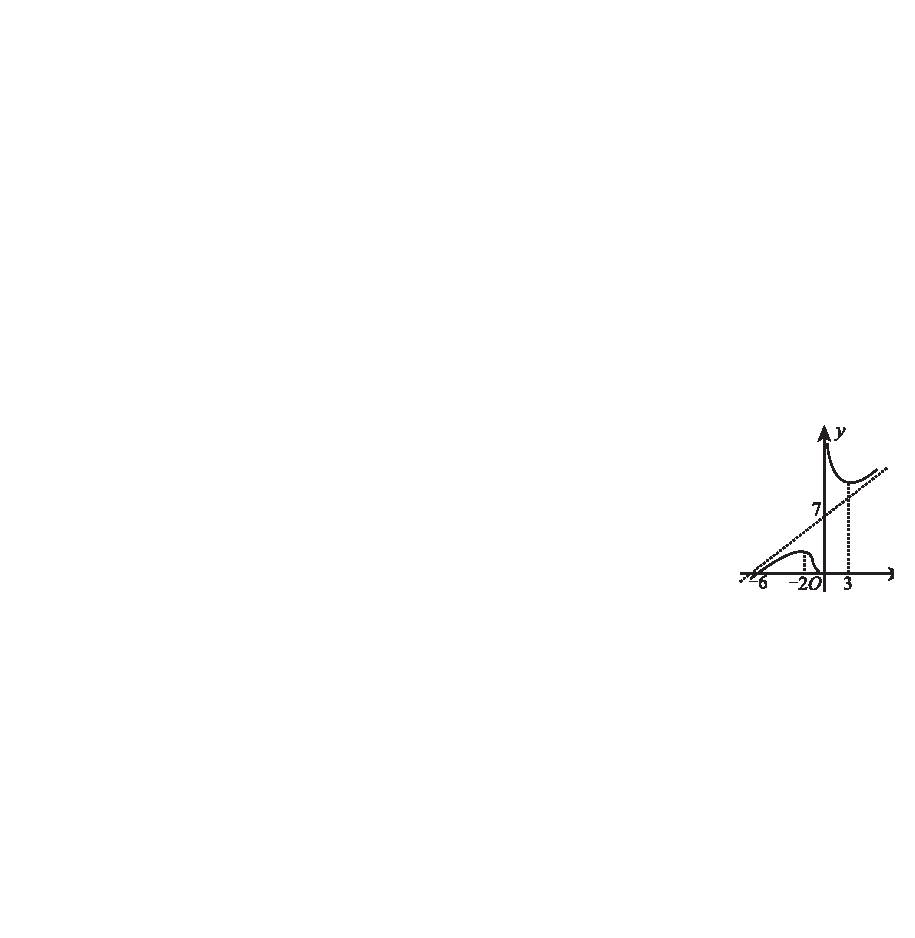
\includegraphics[width=.48\linewidth]{../assets/figures/page-073-10.pdf}\end{center}

八、\(\displaystyle (A^*)^{-1}=\begin{pmatrix}5&-2&-1\\-2&2&0\\-1&0&1\end{pmatrix}\)。


九、\(\displaystyle A\) 的列向量组线性无关。理由略。（\(\displaystyle BA(k_1,\allowbreak k_2,\allowbreak \ldots,\allowbreak k_n)^{\mathrm T}=(k_1,\allowbreak k_2,\allowbreak \ldots,\allowbreak k_n)^{\mathrm T}=0\Rightarrow k_1=k_2=\cdots=k_n=0\)。）


十、（1）\(\displaystyle a=\dfrac{\displaystyle 5}{\displaystyle 3}\) 或 \(\displaystyle \dfrac{\displaystyle 7}{\displaystyle 3}\)。（2）\(\displaystyle \dfrac{\displaystyle 1}{\displaystyle 2}\ln3\)。


十一、【同试卷 IV 第十一题】

\end{document}
